\section{Results}
\label{sec:results}

We report results by hypothesis: difficulty shape (H1, \secref{sec:res_h1}), difficulty variance and lifetime (H3, \secref{sec:res_h3}), and seed noise (H2, \secref{sec:res_h2}). We close with the real leaderboard trajectories (\secref{sec:res_history}).

\subsection{H1: Difficulty shape barely moves the saturation point}
\label{sec:res_h1}

\begin{figure}[t]
    \centering
    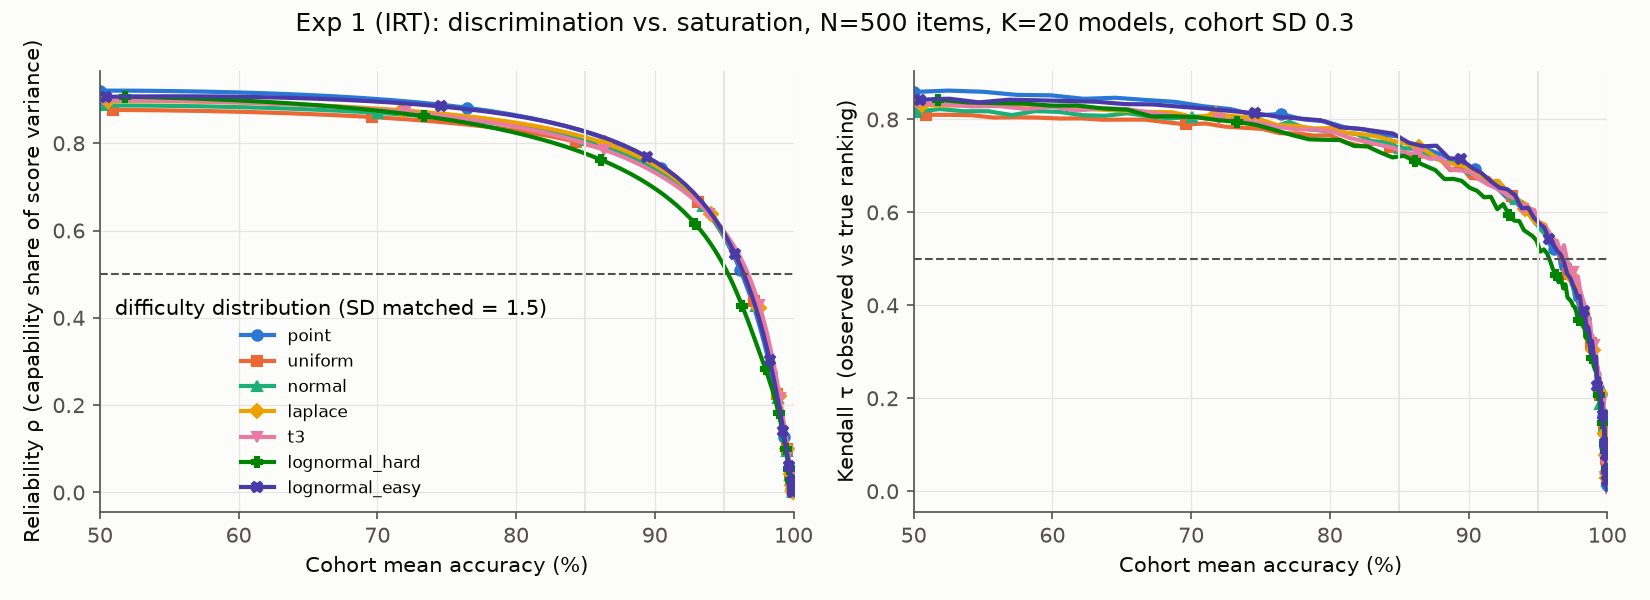
\includegraphics[width=0.95\linewidth]{figures/exp1_discrimination_vs_accuracy.png}
    \caption{{\bf Discrimination \versus saturation in the IRT model} ($\Nitems = 500$ items, $\Kmod = 20$ models, cohort SD $\sigc = 0.3$, difficulty SD matched at 1.5 logits). \figleft{} Reliability $\rho$ (capability share of score variance). \figright{} Kendall $\tau$ between observed and true rankings. The dashed line marks 0.5. All seven difficulty shapes follow nearly the same curve and cross 0.5 between 95\% and 97\% accuracy; the hard-tailed log-normal (dark green) crosses first.}
    \label{fig:exp1_curves}
\end{figure}

\begin{table}[t]
    \centering
    \resizebox{\textwidth}{!}{%
    \begin{tabular}{@{}lccccccc@{}}
        \toprule
        \textbf{Setting} & \textbf{point} & \textbf{uniform} & \textbf{normal} & \textbf{Laplace} & \textbf{$t_3$} & \textbf{\lnhard} & \textbf{\lneasy} \\
        \midrule
        Base ($\Nitems{=}500$, $\sigc{=}0.3$, SD${=}1.5$) & 96.4 & {\bf 96.6} & 96.5 & 96.2 & 96.1 & 95.2 & 96.5 \\
        \midrule
        $\Nitems = 100$ items          & {\bf 84.5} & 82.1 & 80.1 & 80.6 & 80.8 & 79.1 & 84.4 \\
        $\Nitems = 2000$ items         & {\bf 99.0} & {\bf 99.0} & {\bf 99.0} & {\bf 99.0} & 98.8 & 98.5 & {\bf 99.0} \\
        Tight cohort $\sigc = 0.15$    & {\bf 87.5} & 86.4 & 85.0 & 84.4 & 85.0 & 83.1 & {\bf 87.5} \\
        Wide cohort $\sigc = 0.6$      & {\bf 99.0} & {\bf 99.0} & {\bf 99.0} & {\bf 99.0} & 98.9 & 98.5 & {\bf 99.0} \\
        Wide difficulties SD $= 3$     & 96.4 & {\bf 96.7} & 95.7 & 94.5 & 94.8 & 92.4 & 96.5 \\
        Guessing $c = 0.25$            & 96.5 & {\bf 96.6} & 96.4 & 96.0 & 96.0 & 94.8 & 96.5 \\
        \bottomrule
    \end{tabular}
    }
    \caption{{\bf Saturation accuracy $\astar$ (cohort mean accuracy, \%, at which $\rho < 0.5$) in the IRT model.} Values are means over 20 item draws; difficulty SD is matched within each row. Higher means the benchmark discriminates longer; the latest-saturating shape in each row is in {\bf bold}. Shape moves $\astar$ by about 1.5 points in the base setting, and the heavy hard tail (\lnhard) saturates {\em earliest} in every row. In contrast, item count ($\Nitems$) and cohort spread ($\sigc$) move $\astar$ by 15--20 points.}
    \label{tab:astar}
\end{table}


\para{In the controlled model, all shapes saturate together.} \Figref{fig:exp1_curves} shows reliability and Kendall $\tau$ as the cohort moves toward the ceiling. The seven curves are nearly indistinguishable until about 90\% accuracy and cross $\rho = 0.5$ within a narrow window. \Tabref{tab:astar} gives the saturation accuracy $\astar$: in the base setting it ranges from 95.2\% to 96.6\%. Using Kendall $\tau < 0.5$ instead gives $\astar = 95.7$--96.9\% for every shape. The ordering is the opposite of H1. Uniform is among the latest to saturate (96.6\%), and the shape with a long hard tail (\lnhard) is the {\em first} to saturate in every setting, by 1--4 points.

\para{Item count and cohort spread move the saturation point by 15--20 points.} The rows of \tabref{tab:astar} vary one factor at a time. Cutting the benchmark to 100 items lowers $\astar$ to 79--85\%, and growing it to 2{,}000 items raises it to 98.5--99\%. Halving the cohort spread to $\sigc = 0.15$ lowers $\astar$ to 83--88\%, and doubling it to 0.6 raises it to 98.5--99\%. The 85\%-\versus-95\% contrast predicted by H1 therefore does appear, but along the axes of benchmark size and cohort tightness, not shape. Adding a 25\% guessing floor changes $\astar$ by at most 0.4 points. Only when the difficulty distribution is very wide (SD $= 3$) do shapes spread out more (92.4--96.7\%), and again the hard tail is worst.

\para{Shape does affect lifetime, but in the opposite direction.} Measured as the length of the ability axis with $\rho \ge 0.5$, uniform has the longest lifetime among matched-variance shapes: 9.0 logits in the base setting \versus 8.2 for \lnhard, and 12.5 \versus 9.2 at SD $= 3$ (\tabref{tab:lifetime_app} in the appendix).

\begin{figure}[t]
    \centering
    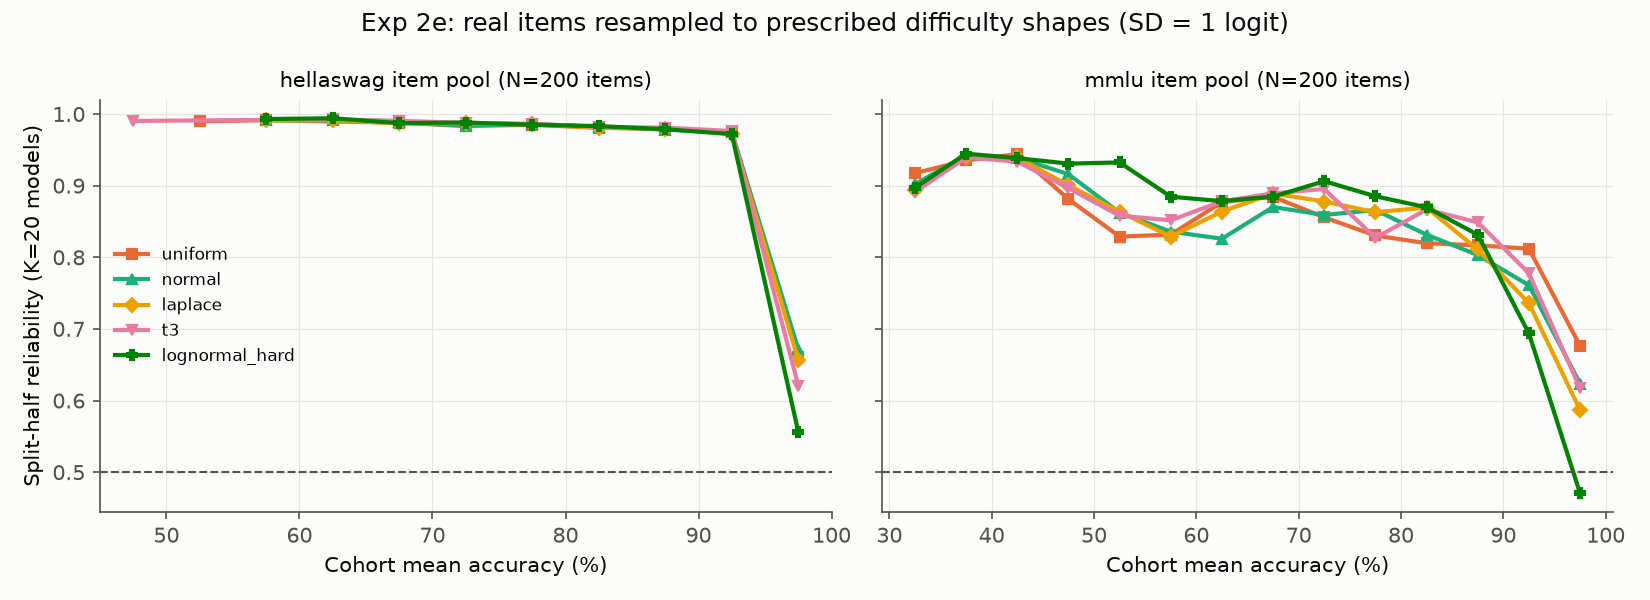
\includegraphics[width=0.95\linewidth]{figures/exp2_resampled_shapes.png}
    \caption{{\bf Real items resampled into prescribed difficulty shapes} (200 items, SD 1 logit, $\Kmod = 20$ held-out real LLMs). \figleft{} \hellaswag pool: all shapes are near-perfectly reliable up to 93\% accuracy and drop together above 95\%. \figright{} \mmlu pool: shapes differ by less than replicate noise below 90\%; above 95\%, uniform holds best (0.68) and the heavy hard tail is the only shape to fall below 0.5.}
    \label{fig:resampled}
\end{figure}

\begin{table}[t]
    \centering
    \small
    \begin{tabular}{@{}llcccc@{}}
        \toprule
        & & \multicolumn{4}{c}{\textbf{Cohort mean accuracy}} \\
        \cmidrule(lr){3-6}
        \textbf{Item pool} & \textbf{Shape} & 80--85\% & 85--90\% & 90--95\% & 95--100\% \\
        \midrule
        \multirow{5}{*}{\mmlu} & uniform              & 0.82 & 0.82 & {\bf 0.81} & {\bf 0.68} \\
                               & normal               & 0.83 & 0.80 & 0.76 & 0.62 \\
                               & Laplace              & {\bf 0.87} & 0.80 & 0.74 & 0.59 \\
                               & $t_3$ (heavy tails)  & {\bf 0.87} & {\bf 0.85} & 0.78 & 0.62 \\
                               & \lnhard (heavy hard tail) & {\bf 0.87} & 0.82 & 0.69 & 0.47 \\
        \midrule
        \hellaswag & all five shapes & 0.98 & 0.98 & 0.97 & 0.55--0.62 \\
        \bottomrule
    \end{tabular}
    \caption{{\bf Direct test of H1 with real items.} Mean split-half reliability of 200-item benchmarks resampled from real \mmlu or \hellaswag items into prescribed difficulty shapes (SD 1 logit) and scored with real responses of $\Kmod = 20$ held-out models. Best per column in {\bf bold}. Uniform does {\em not} saturate at 85\%; it is the most robust shape above 90\% accuracy on \mmlu, and the heavy hard tail is the least robust.}
    \label{tab:resampled}
\end{table}


\para{Real items reproduce the null.} \Figref{fig:resampled} and \tabref{tab:resampled} test H1 directly: we build 200-item benchmarks from real \mmlu and \hellaswag items with prescribed difficulty shapes and score them with real model responses. On \mmlu, the uniform benchmark keeps $\rho = 0.81$ at 90--95\% accuracy and 0.68 above 95\%; it is the most robust shape near the ceiling, not the least. The hard-tailed benchmark is the only one that drops below 0.5 (0.47 above 95\%). On \hellaswag, all five shapes stay at $\rho \ge 0.97$ up to 95\% and fall together to 0.55--0.62 above it. Neither pool shows uniform benchmarks failing at 85\%.

\subsection{H3: Difficulty variance predicts lifetime only at fixed benchmark size}
\label{sec:res_h3}

\begin{figure}[t]
    \centering
    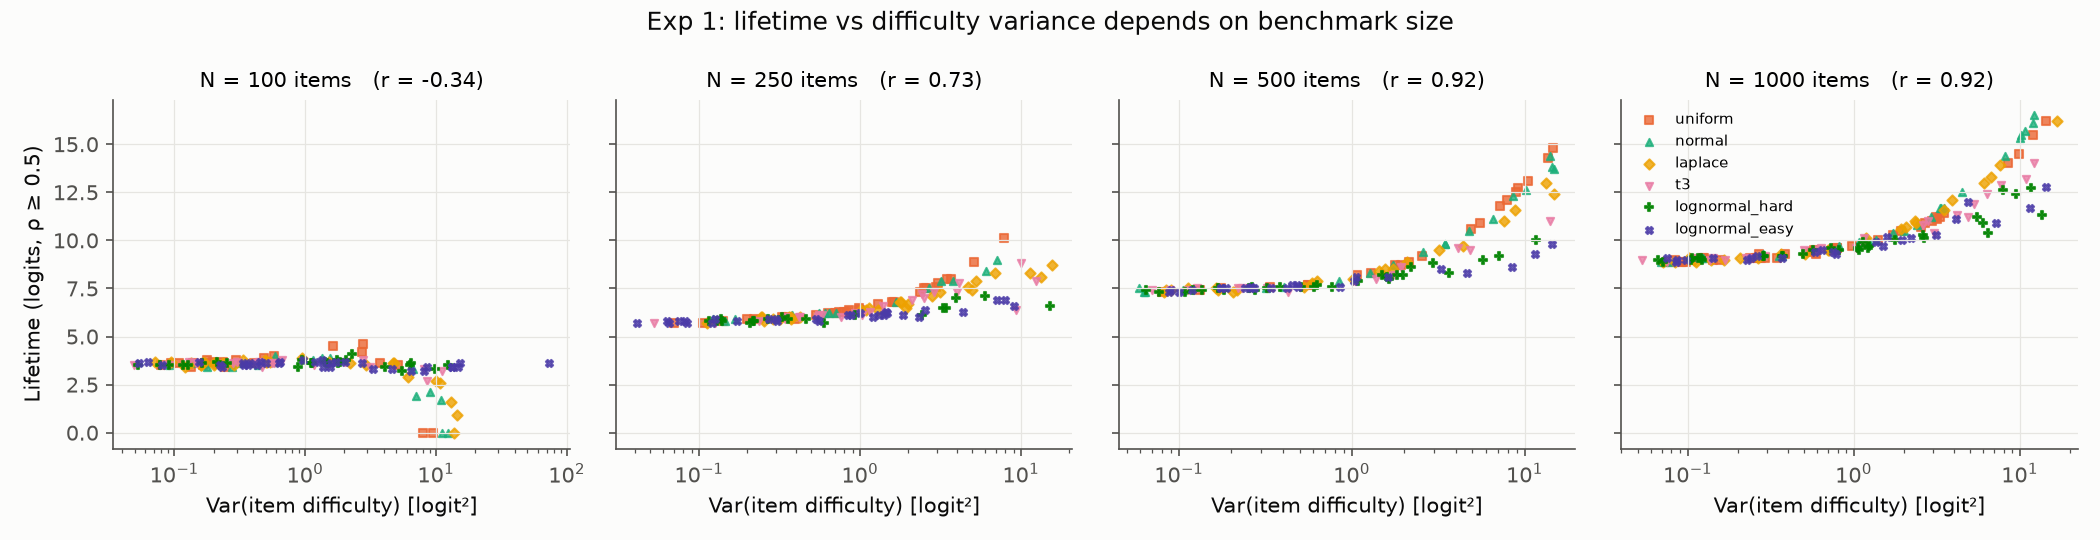
\includegraphics[width=\linewidth]{figures/exp1_lifetime_vs_variance.png}
    \caption{{\bf Lifetime \versus difficulty variance in 600 random IRT benchmarks, split by size.} Lifetime is the length of the ability axis (logits) with $\rho \ge 0.5$. At $\Nitems \ge 500$, more variance means a longer lifetime ($r = 0.92$). At $\Nitems = 100$, the relation reverses ($r = -0.34$): spreading few items over a wide range leaves too few near any one ability level, and some wide 100-item benchmarks never reach $\rho \ge 0.5$. Pooled over sizes, $r = 0.20$.}
    \label{fig:exp1_lifetime}
\end{figure}

\para{In the IRT model, the correlation depends on size.} \Figref{fig:exp1_lifetime} plots lifetime against $\Var(b)$ for 600 random benchmark configurations. Within a fixed size, the relation is strong for large benchmarks: $r = 0.92$ at both $\Nitems = 500$ and $\Nitems = 1000$, and the 90\% difficulty range predicts lifetime even better ($r = 0.96$ at $\Nitems = 500$). It weakens to $r = 0.73$ at $\Nitems = 250$ and reverses to $r = -0.34$ at $\Nitems = 100$. Pooled across sizes, the correlation is only $r = 0.20$ (Spearman 0.27), because size differences dominate lifetime. H3 thus holds in theory, but only within a family of equal-size benchmarks with at least 500 items.

\begin{figure}[t]
    \centering
    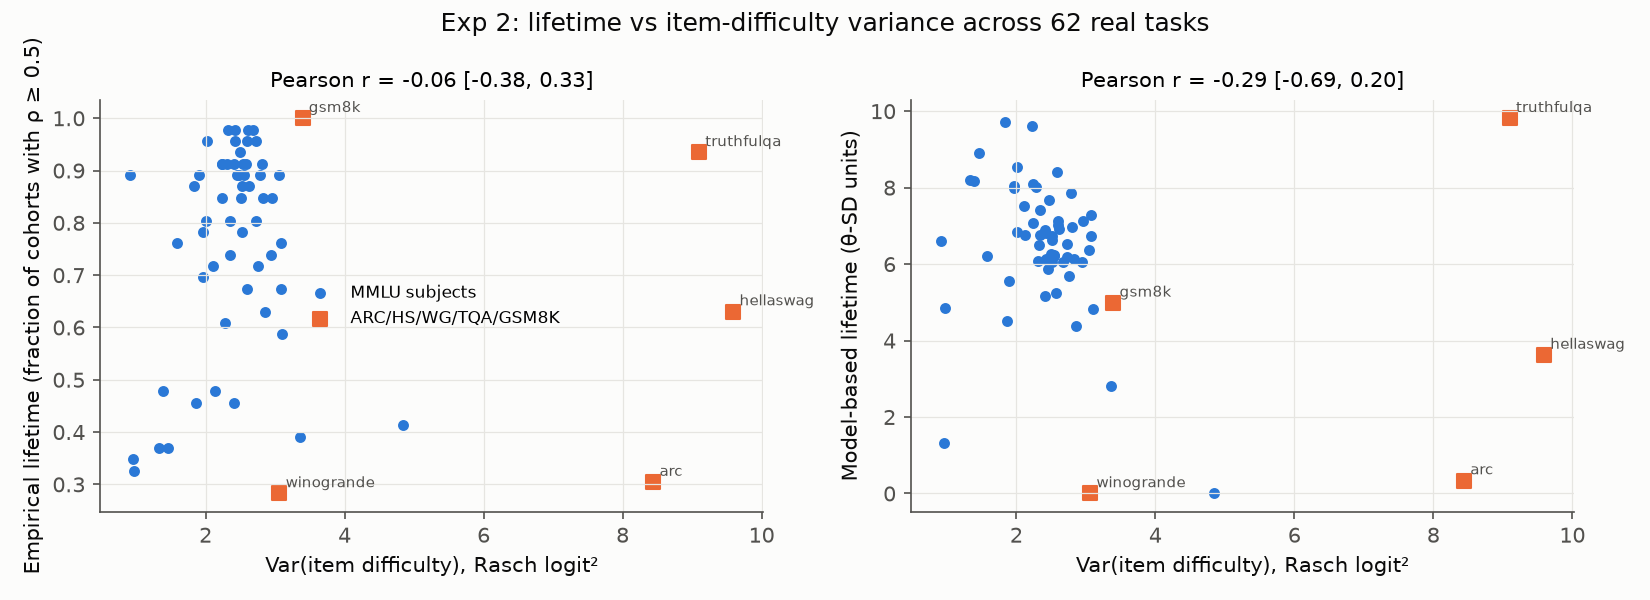
\includegraphics[width=0.95\linewidth]{figures/exp2_lifetime_vs_variance.png}
    \caption{{\bf Lifetime \versus item-difficulty variance across 62 real tasks.} \figleft{} Empirical lifetime (fraction of 20-model cohorts with split-half $\rho \ge 0.5$ on 90-item subsamples). \figright{} Model-based lifetime from each task's fitted Rasch difficulties. Blue: \mmlu subjects; orange: the five other benchmarks. Neither panel shows a positive relation. \hellaswag has the largest $\Var(b)$ but a short lifetime; \gsm has modest $\Var(b)$ but stays discriminative throughout.}
    \label{fig:exp2_lifetime}
\end{figure}

\begin{table}[t]
    \centering
    \resizebox{0.9\textwidth}{!}{%
    \begin{tabular}{@{}lccc@{}}
        \toprule
        \textbf{Lifetime measure} & \textbf{Pearson $r$ [95\% CI]} & \textbf{Spearman} & \textbf{Partial $r$ $\mid$ mean acc.} \\
        \midrule
        Empirical (fraction of cohorts with split-half $\rho \ge 0.5$) & $-0.06$ [$-0.38$, $0.33$] & $\phantom{-}0.08$ & $-0.14$ \\
        Empirical (binomial $\rho$)                                   & $-0.10$ [$-0.45$, $0.30$] & $-0.17$ & $-0.08$ \\
        Model-based (real difficulties, $\theta$-SD units)            & $-0.29$ [$-0.69$, $0.20$] & $-0.35$ & $-0.25$ \\
        \bottomrule
    \end{tabular}
    }
    \caption{{\bf Lifetime \versus item-difficulty variance $\Var(b)$ across 62 real tasks} (220 leaderboard models). Confidence intervals are from 2{,}000 bootstrap resamples. No measure comes close to the hypothesised $r > 0.8$; every interval includes zero. Other variance measures (SD, IQR, 90\% range, $\Var(\mathrm{logit}\,p)$) all give $|r| < 0.3$.}
    \label{tab:exp2corr}
\end{table}


\para{Across real tasks, the correlation vanishes.} \Tabref{tab:exp2corr} and \figref{fig:exp2_lifetime} report the same test on 62 real tasks. Empirical lifetime is uncorrelated with $\Var(b)$ ($r = -0.06$, 95\% CI $[-0.38, 0.33]$), and the model-based lifetime is, if anything, negatively correlated ($r = -0.29$). Controlling for mean accuracy does not change this, and neither do alternative measures of spread ($|r| < 0.3$ for all). Restricting to the 57 \mmlu subjects, which share one format, gives $r = 0.18$ ($p = 0.17$). Two tasks illustrate the gap between variance and lifetime: \hellaswag has the largest difficulty variance yet loses discrimination for the top cohort, whereas \gsm has modest variance yet stays discriminative for every cohort.

\para{Real cohorts saturate on the most saturated tasks.} On 90-item subsamples, real 20-model cohorts rarely exceed a split-half reliability of 0.7 (\figref{fig:exp2_reliability} in the appendix). On the two most saturated tasks the top cohort loses discrimination: \hellaswag drops from a peak of 0.96 for lower cohorts to 0.10 for the top cohort (91\% accuracy), and \winogrande from 0.77 to 0.23 (86\% accuracy). In contrast, \gsm (generative) and \truthfulqa keep high reliability for the top cohort (0.72 and 0.91).

\subsection{H2: Seed noise dominates only for near-tied models on small, near-ceiling test sets}
\label{sec:res_h2}

\para{Seed noise is a fixed fraction of item-sampling noise.} Seed-averaged greedy accuracy on \arce ranges from 59.5\% (Qwen2.5-0.5B) to 97.3\% (Qwen2.5-14B). Across models, the median seed SD of accuracy on 500 items is 0.75 points on \arce (range 0.43--1.83), 0.95 on \arcc (0.43--2.22), and 1.30 on \mmlu (0.68--2.54). Seed variance scales like binomial variance: $\Nitems \cdot \Var_{\text{seed}}(\text{acc}) \approx 0.40 \times \text{acc}(1-\text{acc})$ (median ratio; 0.40 on \arcc, 0.45 on \arce, 0.37 on \mmlu). Option-order seeds therefore add noise equal to roughly 40\% of the noise from sampling the items themselves.

\begin{table}[t]
    \centering
    \resizebox{\textwidth}{!}{%
    \begin{tabular}{@{}llcccccc@{}}
        \toprule
        & & & \multicolumn{2}{c}{\textbf{Seed share}} & \multicolumn{2}{c}{\textbf{Ranking stability (greedy)}} \\
        \cmidrule(lr){4-5} \cmidrule(lr){6-7}
        \textbf{Benchmark} & \textbf{Cohort} & \textbf{Mean acc.} & \textbf{greedy} & \textbf{sampled} & \textbf{Kendall $\tau$} & \textbf{Pair flip prob.} \\
        \midrule
        \mmlu & all 15 & 60\%   & 0.02 & 0.02 & 0.95 & 0.03 \\
        \mmlu & top 6  & 69\%   & 0.10 & 0.10 & 0.90 & 0.06 \\
        \arcc & all 15 & 78\%   & 0.01 & 0.01 & 0.95 & 0.04 \\
        \arcc & top 6  & 88\%   & 0.10 & 0.09 & 0.89 & 0.09 \\
        \arce & all 15 & 90\%   & 0.01 & 0.01 & 0.91 & 0.06 \\
        \arce & top 6  & 96.0\% & {\bf 0.18} & {\bf 0.15} & 0.81 & 0.14 \\
        \bottomrule
    \end{tabular}
    }
    \caption{{\bf Seed noise on natural 500-item benchmarks (15 open LLMs, 10 option-order seeds).} Seed share is the fraction of score variance due to evaluation seeds; Kendall $\tau$ compares a single-seed ranking with the seed-averaged ranking; pair flip probability is the chance that two single-seed runs order a model pair differently. Even for the near-ceiling \arce top-6 cohort (96\% accuracy), seeds explain only 18\% of score variance ({\bf bold}: the largest share). Item-bootstrap upper bounds of the seed share stay below 0.5 for every row (largest: 0.46, \arce top 6).}
    \label{tab:natural}
\end{table}


\para{On full 500-item benchmarks, seeds explain at most 18\% of variance.} \Tabref{tab:natural} shows that seed share grows as the cohort narrows and accuracy rises, from 1--2\% for the full 15-model cohorts to 10\% for the top 6 on \mmlu and \arcc, and 18\% for the \arce top 6 at 96\% accuracy. Rankings are correspondingly stable (single-seed Kendall $\tau \ge 0.81$). The top-1 model is the least stable quantity: across settings, a single seed picks the seed-averaged winner in 40--100\% of cases, and on \arce a single greedy seed finds it only 40\% of the time. Sampling at temperature 1 adds little beyond option order (seed share 0.15 \versus 0.18).

\begin{figure}[t]
    \centering
    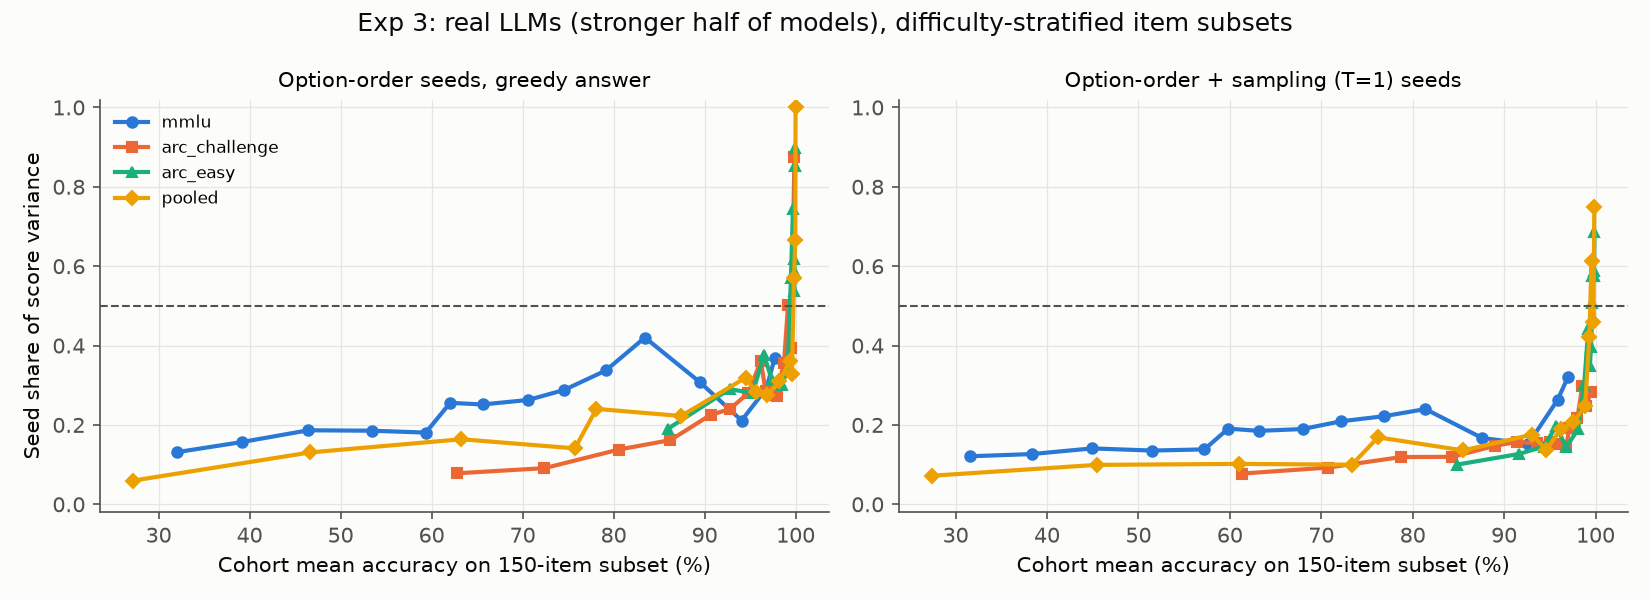
\includegraphics[width=0.95\linewidth]{figures/exp3_seed_share_vs_accuracy.png}
    \caption{{\bf Seed share of score variance \versus cohort accuracy on difficulty-stratified 150-item subsets} (stronger 8 of 15 LLMs; difficulty estimated on the weaker 7). \figleft{} Option-order seeds, greedy answers. \figright{} Option order plus sampling at $T = 1$. Seed share rises steadily with accuracy (Spearman 0.96 greedy, 0.97 sampled) but crosses 0.5 (dashed) only at $\ge 99\%$ accuracy on \arcc and \arce, where nearly every model solves nearly every item.}
    \label{fig:exp3}
\end{figure}

\para{Seed share rises with accuracy but crosses 0.5 only at the very top.} \Figref{fig:exp3} uses difficulty-stratified 150-item subsets. Seed share rises monotonically with cohort accuracy (pooled Spearman $\rho = 0.96$, $p < 10^{-8}$ greedy; $0.97$, $p < 10^{-9}$ sampled). The mean share is 0.46 at accuracy $\ge 90\%$ \versus 0.15 below 80\% (greedy). On \mmlu it peaks at 0.42 (83\% accuracy). On \arcc and \arce it exceeds 0.5 only at $\ge 99.2\%$ accuracy. H2 thus has the right direction but requires a much stronger form of saturation than ``mean accuracy above 90\%''.

\para{Item count again decides.} For the \arce top-6 cohort, the seed share falls from 0.51 at 50 items to 0.45 at 100, 0.32 at 200, and 0.18 at 500 items (\tabref{tab:nitems} in the appendix). Seed noise shrinks as $1/\Nitems$ while the capability gap does not, so large benchmarks rarely let seeds dominate.

\begin{table}[t]
    \centering
    \small
    \begin{tabular}{@{}lcccc@{}}
        \toprule
        \textbf{Benchmark} & \textbf{Top-20 mean} & \textbf{Top-20 SD} & \textbf{Pred.\ seed SD} & \textbf{Pred.\ seed share} \\
        \midrule
        \arc        & 76.6\% & 2.6 pts & 0.78 pts & 0.09 \\
        \hellaswag  & 89.4\% & 1.7 pts & 0.19 pts & 0.01 \\
        \mmlu       & 78.1\% & 1.1 pts & 0.22 pts & 0.04 \\
        \truthfulqa & 73.6\% & 5.0 pts & 0.97 pts & 0.04 \\
        \winogrande & 85.5\% & 1.6 pts & 0.62 pts & {\bf 0.14} \\
        \gsm        & 79.7\% & 3.8 pts & 0.70 pts & 0.03 \\
        \bottomrule
    \end{tabular}
    \caption{{\bf Predicted seed share for the real \leaderboard top-20 (June 2024).} We apply the seed-noise rate fitted in Exp~3 ($\Nitems \cdot \Var_{\text{seed}} \approx 0.40\,\text{acc}(1-\text{acc})$) to each benchmark's size and top-20 score spread. The largest predicted share ({\bf bold}) is 14\%, for the smallest benchmark (\winogrande, 1{,}267 items).}
    \label{tab:crosscheck}
\end{table}


\para{Real leaderboards are far from the seed-dominated regime.} \Tabref{tab:crosscheck} applies the fitted seed-noise rate to the real \leaderboard top-20 as of June 2024. Predicted seed shares range from 1\% (\hellaswag) to 14\% (\winogrande). With 800--14{,}000 items per benchmark, seed noise is small compared with the spread of the frontier, even on benchmarks above 85\% mean accuracy.

\subsection{Real leaderboard trajectories}
\label{sec:res_history}

\begin{figure}[t]
    \centering
    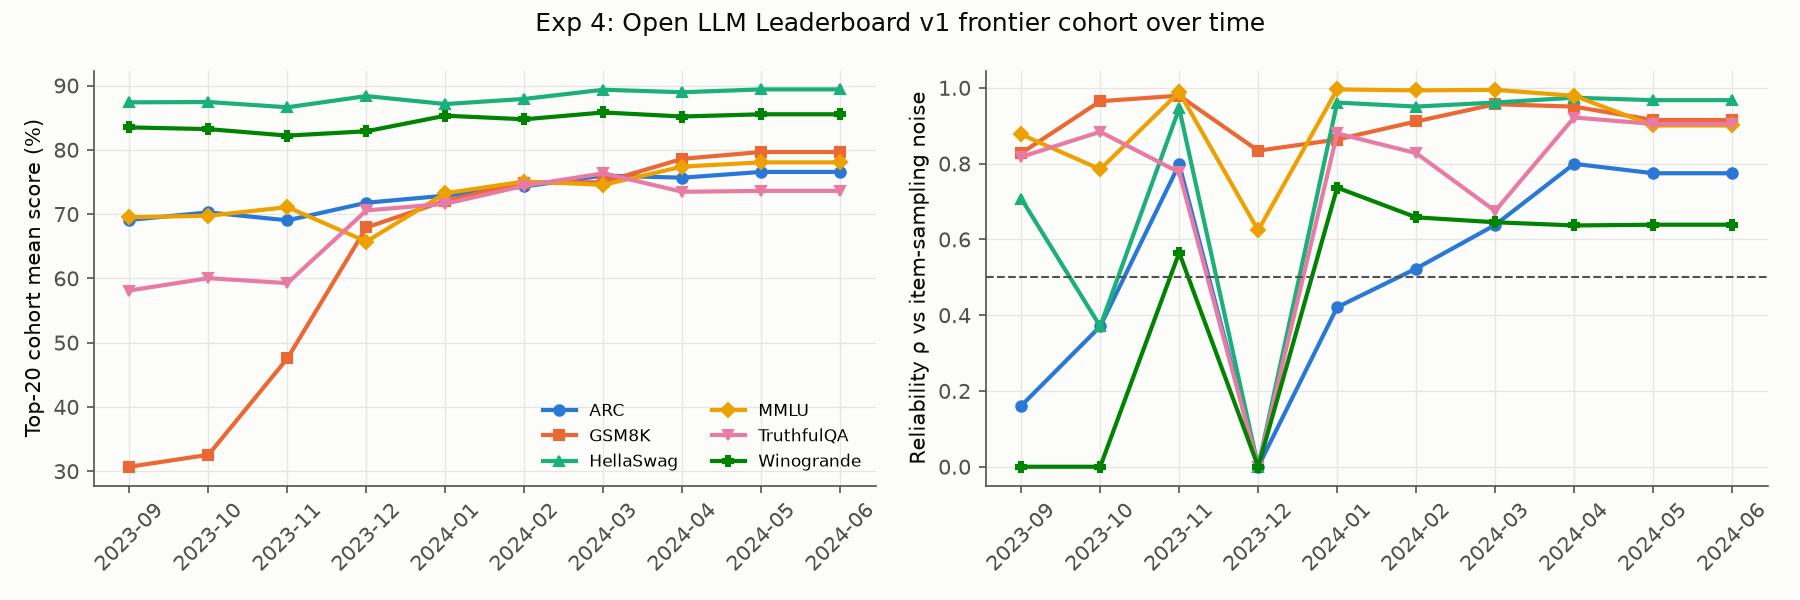
\includegraphics[width=0.95\linewidth]{figures/exp4_leaderboard_history.png}
    \caption{{\bf The \leaderboard frontier cohort (top 20 unique models) by month.} \figleft{} Cohort mean score. \gsm rose fastest (31\% to 80\%), \mmlu rose from 70\% to 78\%, and \hellaswag from 87\% to 89\%. \figright{} Reliability $\rho$ against item-sampling noise. Large benchmarks stay above 0.9 in most months after January 2024; smaller ones (\winogrande, \arc) are less reliable. In December 2023, $\rho \approx 0$ for every benchmark at once because near-duplicate model merges dominated the top 20.}
    \label{fig:exp4}
\end{figure}

\Figref{fig:exp4} shows how the real frontier evolved. Frontier means rose on every benchmark, fastest on \gsm (31\% to 80\%). Reliability against item-sampling noise stayed at or above 0.9 for \hellaswag, \mmlu, \gsm and \truthfulqa in most months after January 2024; \hellaswag and \mmlu have 10k--14k items. The smaller benchmarks were less reliable even at lower accuracy: \winogrande (1{,}267 items) at about 0.64 and \arc at about 0.4--0.8. Most strikingly, in some months (\eg December 2023) $\rho \approx 0$ on {\em every} benchmark at once. In these months the top 20 was dominated by near-duplicate merged models whose scores differed by less than item-sampling noise. This is saturation of the {\em cohort}, not of any benchmark, and it confirms that cohort spread is as important as benchmark design in deciding whether ranks are meaningful.
